% !TeX program = pdflatex
% ============================================================================
%  期刊（目录原表名称）：Lancet Psychiatry
%  期刊（官方标题）    ：The Lancet Psychiatry
%  分级                ：A（自然科学类）
%  出版商              ：Elsevier
%  官方文档类          ：Elsevier elsarticle v3.4 (2024/04/04)
%  文档类来源          ：https://ctan.org/pkg/elsarticle
%  投稿指南            ：https://www.elsevier.com/researcher/author/policies-and-guidelines/latex-instructions
%  文档类许可证        ：LPPL 1.3（类文件未作任何修改）
% ============================================================================
%  这是投稿模板，不是真实论文。标题、作者、单位、摘要、正文、图表和文献
%  都是示例内容，请全部替换为您自己的材料。
%
%  请勿修改随附的 .cls / .sty / .bst 文件；排版由出版商官方文档类负责。
%  编译：latexmk -pdf main.tex
% ============================================================================

\documentclass[preprint,12pt]{elsarticle}
\usepackage{amsmath,amssymb}
\usepackage{graphicx}
\usepackage{booktabs}
\usepackage[hidelinks]{hyperref}

\journal{The Lancet Psychiatry}

\begin{document}

\begin{frontmatter}
\title{A \LaTeX{} Submission Template for \textit{The Lancet Psychiatry}}

\author[a]{First Author\corref{cor1}}
\ead{first.author@example.edu}
\author[b]{Second Author}
\affiliation[a]{organization={Department of Example Science, Example University},
                city={Wuhan}, postcode={430070}, country={China}}
\affiliation[b]{organization={Example Research Institute},
                city={Beijing}, postcode={100190}, country={China}}
\cortext[cor1]{Corresponding author.}

\begin{abstract}
This document demonstrates the official Elsevier \texttt{elsarticle} class
configured for \textit{The Lancet Psychiatry}. It is a template, not a real manuscript:
replace the front matter, body text, figures, tables, and references with
your own material.
\end{abstract}

\begin{keyword}
template \sep \LaTeX \sep Elsevier \sep The Lancet Psychiatry
\end{keyword}
\end{frontmatter}

\maketitle

\section{Introduction}
\label{sec:introduction}
This document is a submission template for \textit{The Lancet Psychiatry}. It is typeset
with the publisher's official \LaTeX{} document class; the class, not this
file, controls the page layout, fonts, and reference formatting. Every piece
of text in this sample---including the author names, affiliations, abstract,
and references---is a placeholder \cite{example2024,example2020}.

Replace the sample material with your own manuscript, but keep the document
class and the front-matter commands unchanged. Check the journal's current
Guide for Authors before submission because article types, word limits, and
reference styles can change.

\section{Using this template}
\label{sec:usage}
\begin{itemize}
  \item Edit \texttt{main.tex} only; the accompanying \texttt{.cls},
        \texttt{.sty}, and \texttt{.bst} files are official files and
        must remain unmodified.
  \item Put figures in \texttt{figures/} and include them with
        \verb|\includegraphics|; a sample vector figure is already provided.
  \item Replace the entries in \texttt{references.bib} and cite them with
        \verb|\cite|. The two entries shipped with the template are examples.
  \item Build the PDF with \texttt{latexmk -pdf main.tex}.
\end{itemize}

\section{Mathematics, tables, and figures}
\label{sec:elements}
Inline mathematics such as $E = mc^2$ and displayed equations are supported:
\begin{equation}
  \int_{-\infty}^{\infty} e^{-x^{2}}\,\mathrm{d}x = \sqrt{\pi}.
  \label{eq:gaussian}
\end{equation}

\begin{table}[t]
  \centering
  \caption{An example table typeset with \texttt{booktabs}. Replace it with your own data.}
  \label{tab:example}
  \begin{tabular}{lcc}
    \toprule
    Item & Value & Unit \\
    \midrule
    Alpha & 1.0 & a.u. \\
    Beta  & 2.0 & a.u. \\
    \bottomrule
  \end{tabular}
\end{table}

\begin{figure}[t]
  \centering
  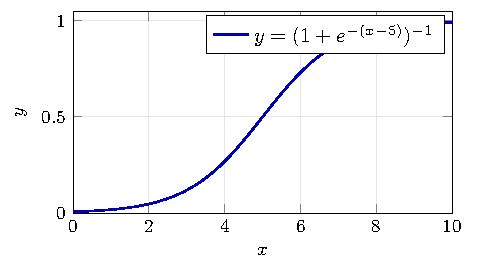
\includegraphics[width=0.62\linewidth]{figures/example-figure}
  \caption{An example vector figure. Replace the file in \texttt{figures/} with your own artwork.}
  \label{fig:example}
\end{figure}

\section{Conclusion}
\label{sec:conclusion}
Replace this paragraph with the conclusion of your manuscript. The template
is intentionally minimal: journal-specific requirements should be taken from
the current author guidelines rather than added as local formatting hacks.

\section*{Declaration of competing interest}
The authors declare that they have no known competing financial interests or
personal relationships that could have appeared to influence this work.

\section*{Data availability}
Data sharing is not applicable to this template article.

\bibliographystyle{elsarticle-num}
\bibliography{references}

\end{document}
